\subsection{Style Tab}
\label{sec:osgview_style}

\begin{figure}[H]
   \center
    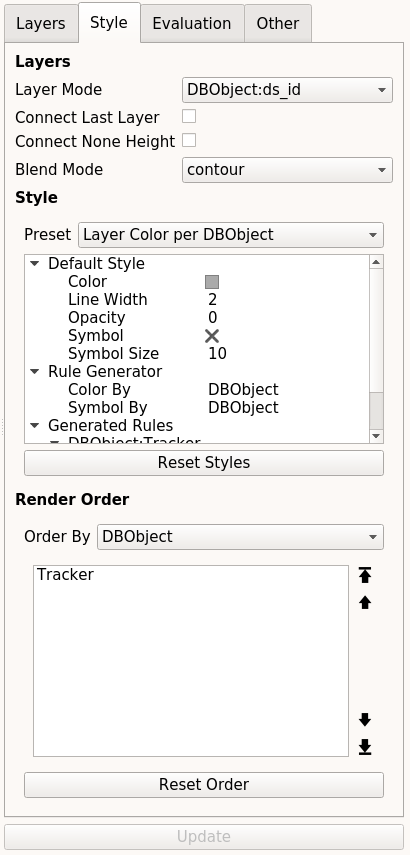
\includegraphics[width=8cm,frame]{../screenshots/osgview_style_tab.png}
  \caption{OSG View Style tab}
\end{figure}

In the 'Style' tab, several elements exist:

\begin{itemize}
 \item Layer Mode: Defines how layers are generated. Please refer to Section \nameref{sec:layer_mode} for details.
 \item Connect Last Layer: Whether grouped target reports in the last layer should be connected using lines
 \item Connect None Height: If groups are connected, whether target reports with not height information should be connected
 \item Blend Mode: Defines the drawing blend mode, allowing clearer symbols (contour) or colors (src-over).
 \item Style: Defines how geometry is styled. Please refer to Section \nameref{sec:style} for details.
 \item Render Order: Defines the drawing order of DBObjects. To bottom one is drawn first, the top one last (over all others)
 \item Update button: Triggers a redraw or reload of the geometry, becomes available after a change if needed.
\end{itemize} 

\subsubsection{Layer Mode}
\label{sec:layer_mode}

In this selection the way layers are generated can be changed. \\\\

The following items can be present in the list:\\

\begin{itemize}
 \item DBObject: DBObject type, e.g. Radar, MLAT, ...
 \item ds\_id: Data source identifier, e.g Radar1, Radar2, ARTAS
 \item callsign: Mode S Target Identification
 \item target\_addr: Mode S Target Address
 \item track\_num: Track number (local or system)
 \item mode3a\_code: Mode 3/A code
 \item UTN: Unique Target Number, only available if association information is present
\end{itemize}
\ \\

The layer mode defines what layers are generated, e.g. for 'A' only layers for all values of 'A' are created, for 'A:B' layers for all values of 'A' are created, each with sub-layers for all values of 'B'. In this case, 'A' is the parent, 'B' is the child. \\\\

If no values exist in the data for a layer, this data is grouped in the layer 'None'.\\\\

The following modes exist: \\

\begin{itemize}
 \item DBObject
 \item DBObject:ds\_id
 \item DBObject:ds\_id:callsign
 \item DBObject:ds\_id:target\_addr
 \item DBObject:ds\_id:track\_num
 \item DBObject:ds\_id:mode3a\_code
 \item UTN:DBObject
 \item UTN:DBObject:ds\_id
 \item UTN:DBObject:ds\_id:target\_addr
 \item UTN:DBObject:ds\_id:track\_num
 \item UTN:DBObject:ds\_id:mode3a\_code
 \item callsign:DBObject
 \item callsign:DBObject:ds\_id 
 \item mode3a\_code:DBObject
 \item mode3a\_code:DBObject:ds\_id
 \item target\_addr:DBObject
 \item target\_addr:DBObject:ds\_id
\end{itemize}
\  \\

Please note that the UTN layer modes only exist when association information is present. \\

Please also note that after a change in the Layer mode a redraw has to be triggered before the changes take effect. \\

As examples, a few values for the Layer mode are listed. \\

\paragraph{DBObject:ds\_id}

In this layer mode the DBObject name is used to create the first layer, with sub-layers for each data source. This is the default mode.

\begin{figure}[H]
    \center
    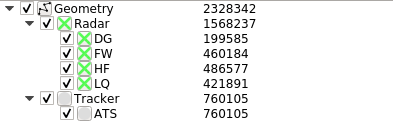
\includegraphics[width=8cm,frame]{../screenshots/osgview_group_dbo_ds.png}
  \caption{OSG View layer mode DBObject:ds\_id}
\end{figure}

\paragraph{mode3a\_code:DBObject}

In this layer mode the Mode 3/A code is used to create the first layer, with sub-layers for each DBObject.

\begin{figure}[H]
\center
    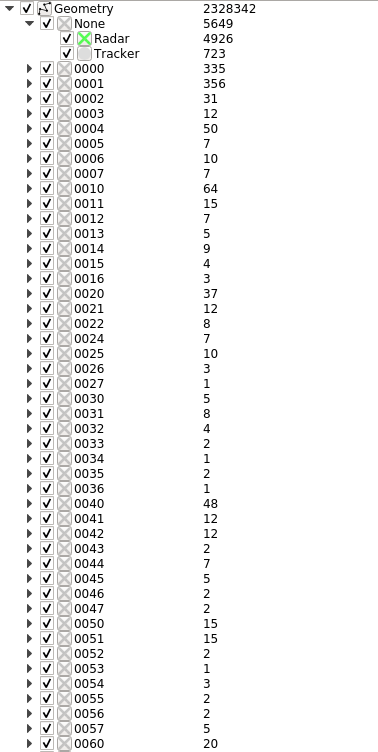
\includegraphics[width=8cm,frame]{../screenshots/osgview_group_ma_dbo.png}
  \caption{OSG View layer mode mode3a\_code:DBObject}
\end{figure}

\paragraph{UTN:DBObject}

In this layer mode the UTN is used to create the first layer, with sub-layers for each DBObject. All target reports without a UTN (not used by ARTAS) are grouped into layer 'None'.  \\

An example of this mode is shown in the styling section.


\subsubsection{Connect Last Layer \& Connect None Height}

If the 'Connect Last Layer' checkbox is set, connection lines between all target reports in the last layer are drawn, except for the 'None' layer. \\

Please note that connection lines for target reports with a time-of-day difference larger than 5 minutes will be omitted. \\

\includegraphics[width=0.5cm]{../../data/icons/hint.png} If this is activated for a Layer mode in which the last layer is not target-specific, this will lead to a sub-optimal representation. \\

This mode (normally) makes sense in one of the following Layer modes:

\begin{itemize}
 \item DBObject:ds\_id:callsign
 \item DBObject:ds\_id:target\_addr
 \item DBObject:ds\_id:track\_num
 \item UTN:DBObject:ds\_id:target\_addr
 \item UTN:DBObject:ds\_id:track\_num
 \item callsign:DBObject:ds\_id 
 \item target\_addr:DBObject:ds\_id
\end{itemize}
\  \\

\begin{figure}[H]
    \hspace*{-2.5cm}
    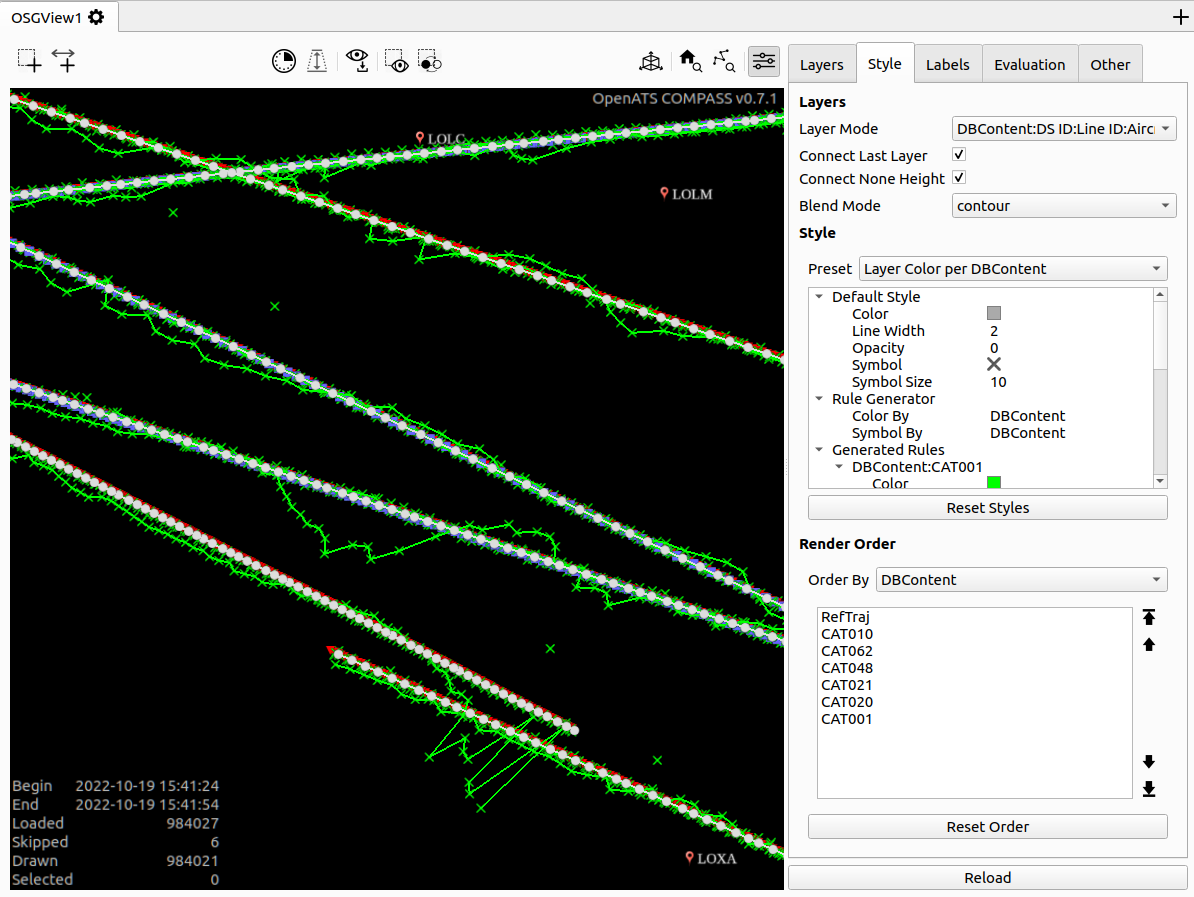
\includegraphics[width=19cm,frame]{../screenshots/osgview_connect_lines.png}
  \caption{OSG View Data with lines}
\end{figure}

If the height information is used (3D view) and if target reports without height information are connected, the lines clutter the display. The 'Connect None Height' checkbox allows to set the behaviour. \\

Please \textbf{note} that changes both these values requires a manual redraw using the 'Redraw' button.

\subsubsection{Style}
\label{sec:style}

There exist 3 main elements for styling:
\begin{itemize}
 \item Preset drop-down menu: Selects currently active style
 \item Style configuration area: Area below the preset menu, allows configuration of the current style
 \item Reset Styles button: Clears all style presets to their default values
\end{itemize}
\  \\

Each style can be composed of 3 elements:
\begin{itemize}
 \item Default Style: Base style which sets the basic styling for all data
 \item Rule Generator: Generated e.g. layer-specific specific rules
 \item Generated Rules: Rules which which override the Default Style
\end{itemize}
\  \\

\includegraphics[width=0.5cm]{../../data/icons/hint.png} Please note that some style presets (e.g. layer style per callsign, target\_addr, track\_num, mode3a\_code) generate lots of different (persistent) styling rules, which decreases startup speed. After using such styles it is possible to reset the styles using the 'Reset Styles' button to increase application startup speed. \\

There are two types of style presets:
\begin{itemize}
 \item Layer-based presets: Perform styling per layer
 \item Target report based presets: Set symbol color per data variable value
\end{itemize}
\  \\

\paragraph{Layer-based Style Presets}
The following layer-based style presets exist:
\begin{itemize}
 \item Default: All data is shown in the same style
 \item Layer Color per DBObject: Style is defined by DBObject type
 \item Layer Color per UTN: Style is defined by UTN value
 \item Layer Color per callsign: Style is defined by callsign value
 \item Layer Color per ds\_id: Style is defined by data source
 \item Layer Color per mode3a\_code: Style is defined by Mode 3/A code
 \item Layer Color per target\_addr: Style is defined by Mode S Target Address
 \item Layer Color per track\_num: Style is defined by track number
\end{itemize}
\  \\

Please note that after changing the style to one of these value a redraw has to be triggered. \\

\includegraphics[width=0.5cm]{../../data/icons/hint.png} Please also note that for such presets the data from which the style is derived has to be present in the Layer mode, otherwise the layer is styled with a common base style.

\paragraph{Target Report based Style Presets}
The following Target report based style presets exist:
\begin{itemize}
 \item Color by ADS-B MOPS: Color is defined by the ADS-B MOPS version of the transponder
 \item Color by ADS-B Position Quality: Color is defined by the ADS-B NUCp/NACp value of the target report
 \item Color by Flight Level: Color is defined by the Mode C code/Flight level
 \item Color by Speed: Color is defined by groundspeed value
 \item Color by Track Angle: Color is defined by direction of movement value
 \item Color by Tracker Detection Type: Color is defined by detection type (PSR, SSR, Combined, ...)
\end{itemize}
\  \\

Please note that after changing the style to one of these value a reload has to be triggered. \\

\subsubsection{Customized Styling}

While the presets come with (mostly) reasonable default values, adaptation can be performed by clicking on the value that should be changed, either in the Default Style or the Generated rules. Any changes are applied immediately to the geometry.

\subsubsection{Style Examples}

To give a few examples, some interesting Layer modes and Style preset combinations are given:

\begin{figure}[H]
    \hspace*{-2.5cm}
    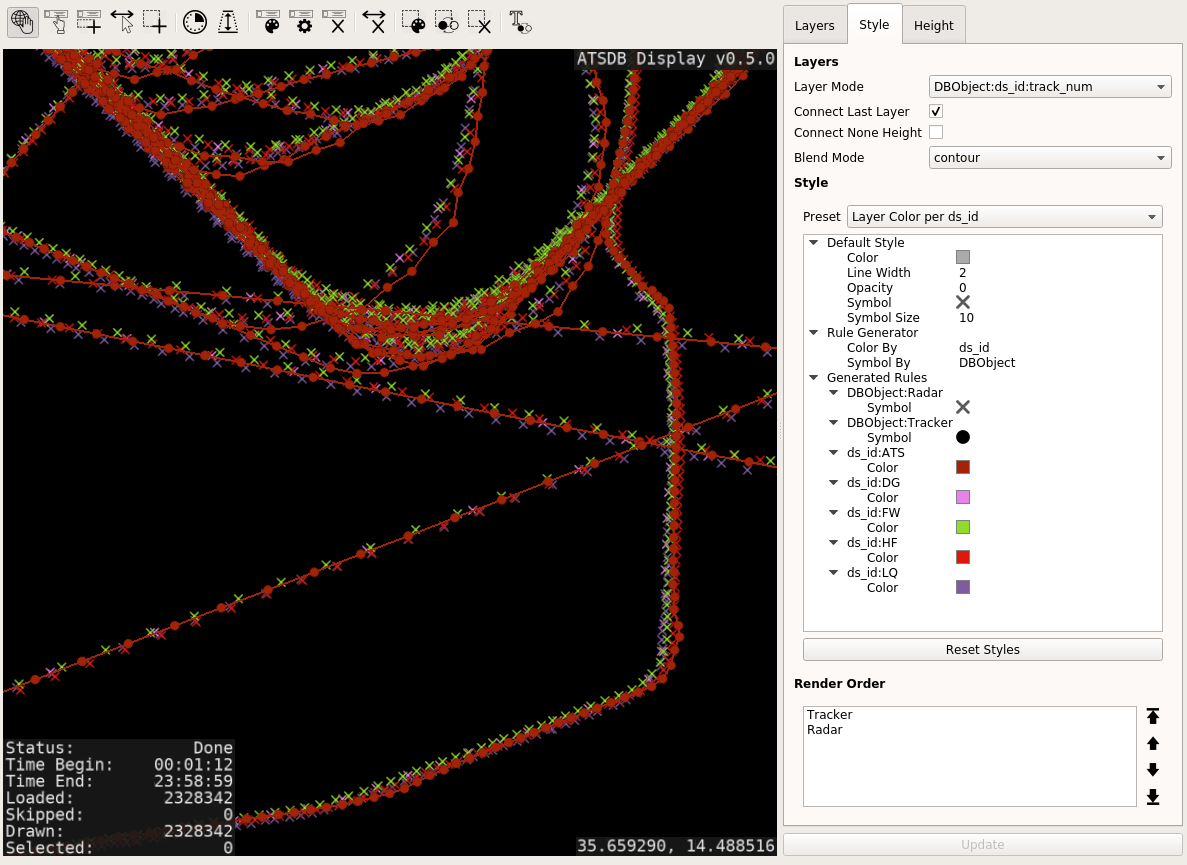
\includegraphics[width=19cm,frame]{../screenshots/osgview_style_ds_id.png}
  \caption{OSG View Layer color per ds\_id}
\end{figure}

\begin{figure}[H]
    \hspace*{-2.5cm}
    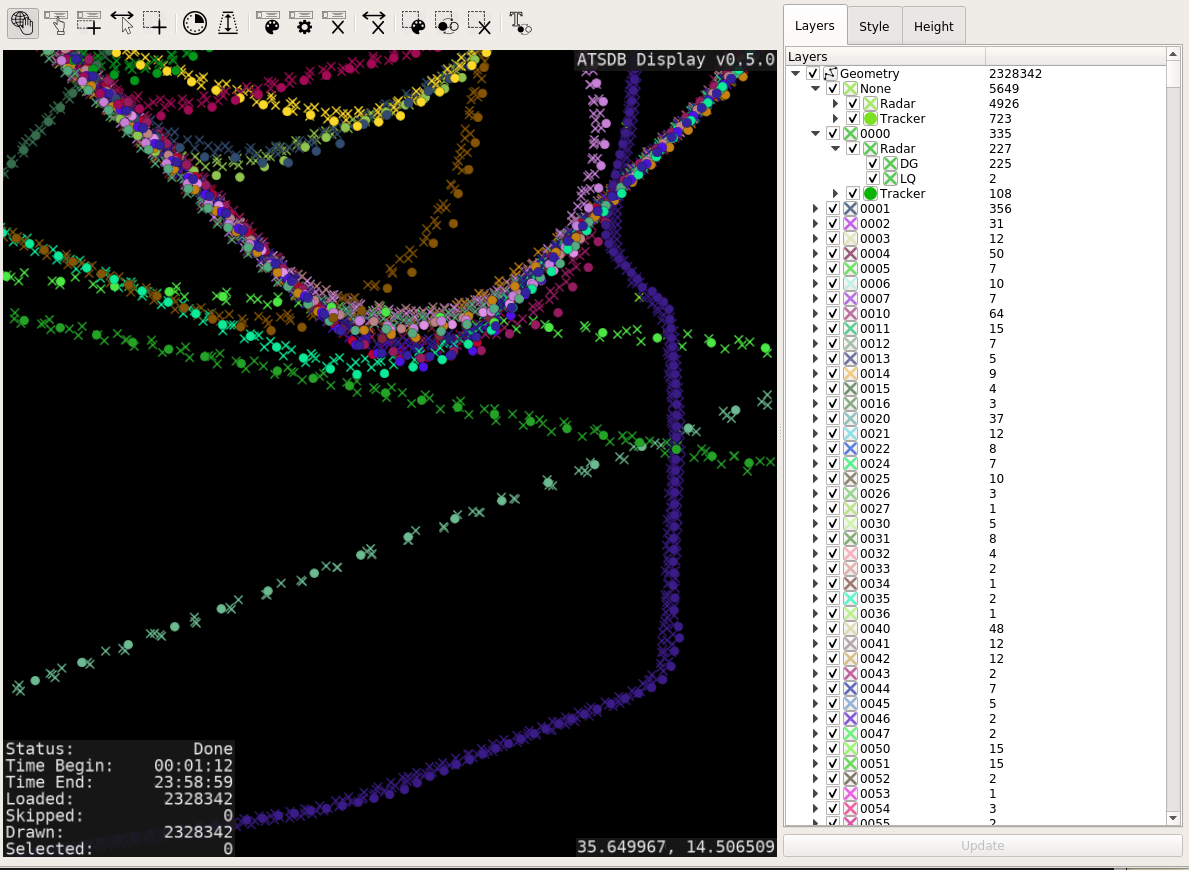
\includegraphics[width=19cm,frame]{../screenshots/osgview_style_mode3a_code.png}
  \caption{OSG View Layer color per mode3a\_code}
\end{figure}

\begin{figure}[H]
    \hspace*{-2.5cm}
    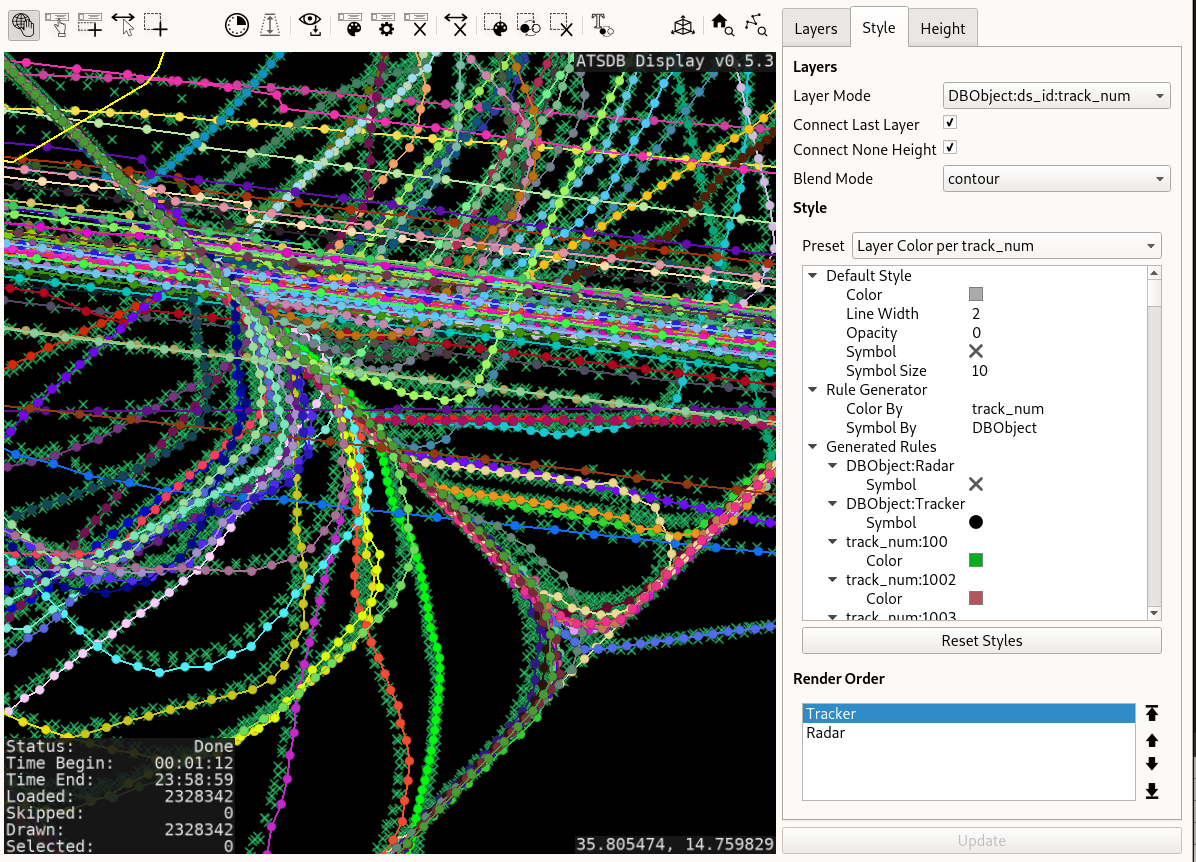
\includegraphics[width=19cm,frame]{../screenshots/osgview_style_track_num.png}
  \caption{OSG View Layer color per track\_num}
\end{figure}

\begin{figure}[H]
    \hspace*{-2.5cm}
    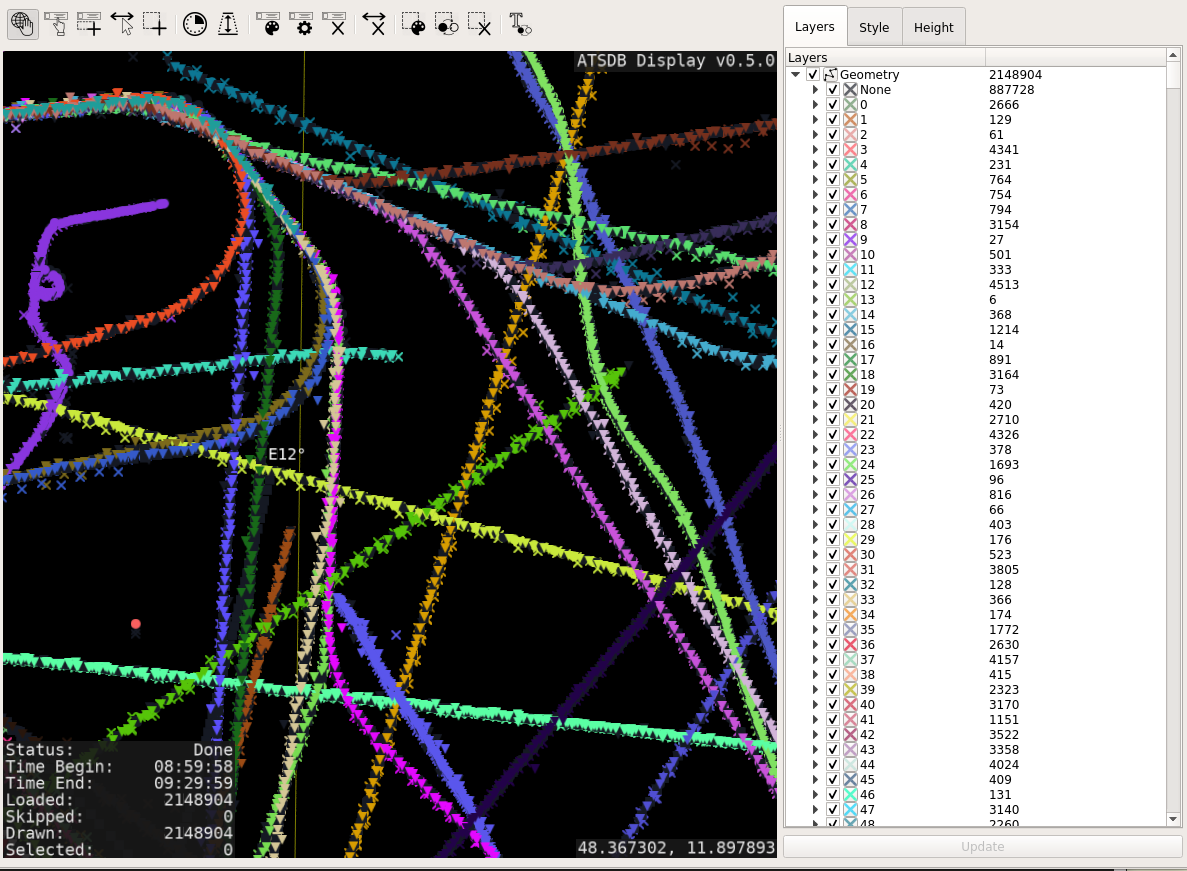
\includegraphics[width=19cm,frame]{../screenshots/osgview_style_utn.png}
  \caption{OSG View Layer color per UTN}
\end{figure}

\begin{figure}[H]
    \hspace*{-2.5cm}
    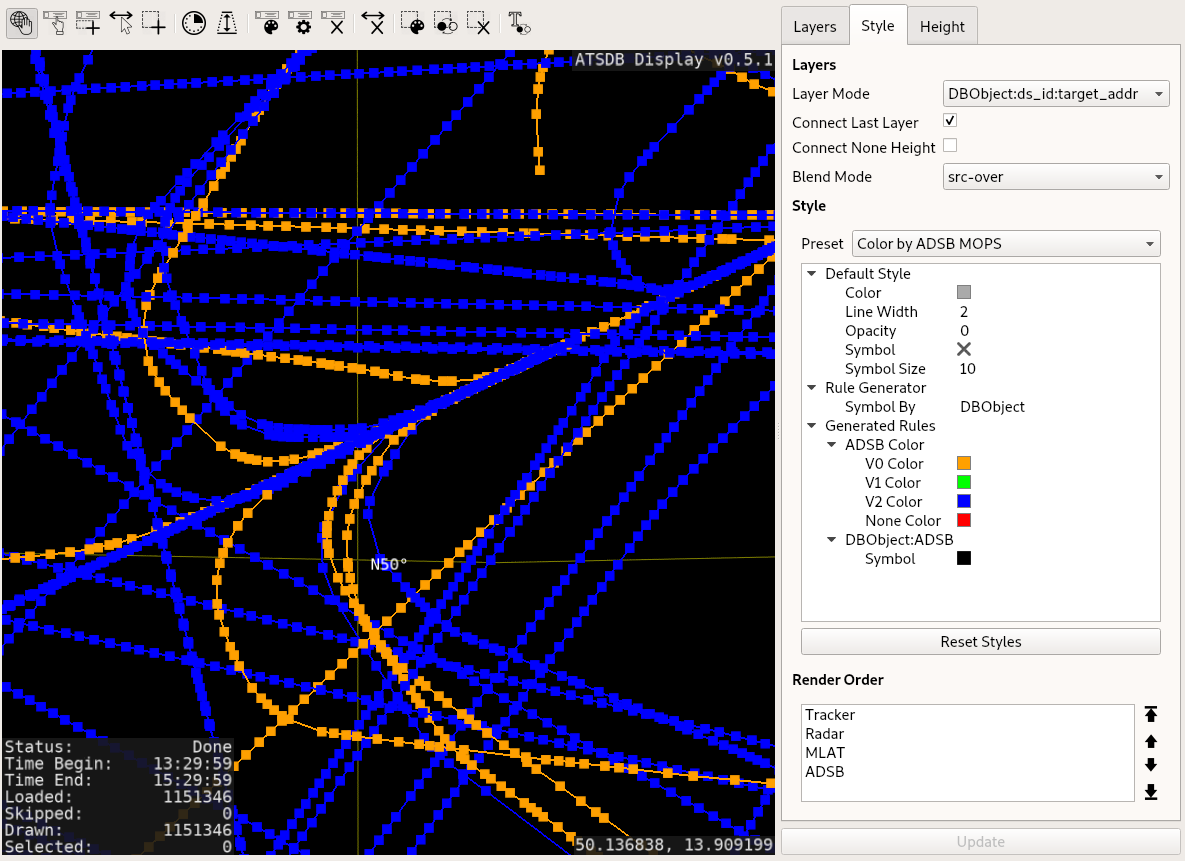
\includegraphics[width=19cm,frame]{../screenshots/osgview_style_adsb_mops.png}
  \caption{OSG View Color by ADS-B MOPS version}
\end{figure}

\begin{figure}[H]
    \hspace*{-2.5cm}
    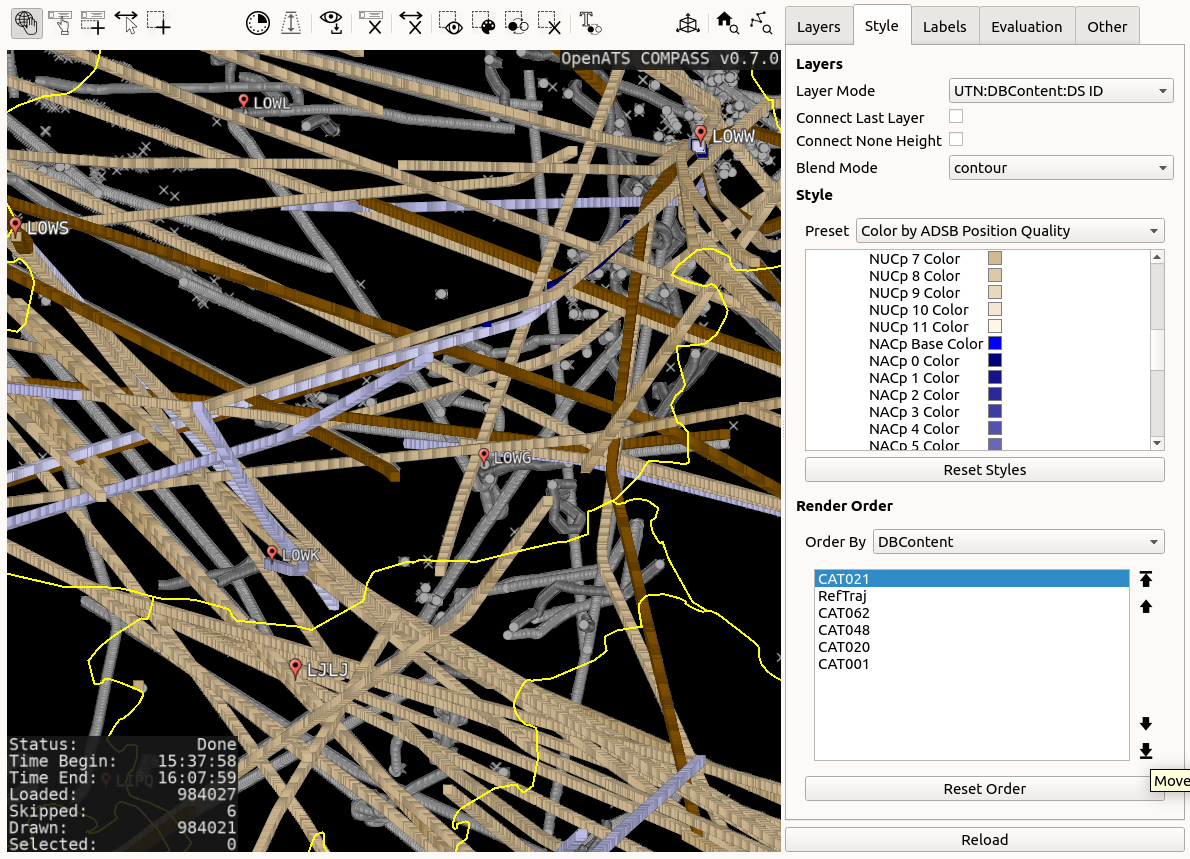
\includegraphics[width=19cm,frame]{../screenshots/osgview_style_adsb_position_qual.png}
  \caption{OSG View Color by ADS-B position quality}
\end{figure}

\begin{figure}[H]
    \hspace*{-2.5cm}
    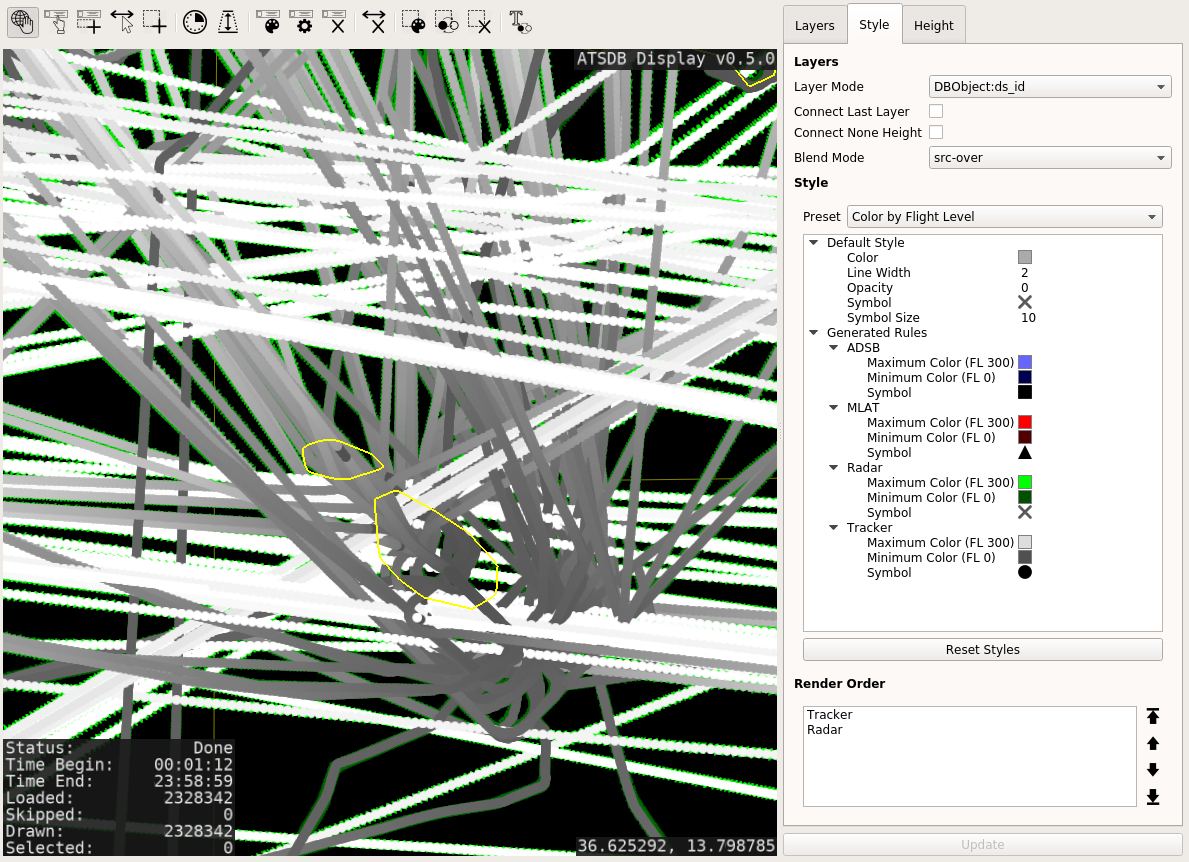
\includegraphics[width=19cm,frame]{../screenshots/osgview_style_flight_level.png}
  \caption{OSG View Color by flight level}
\end{figure}

\begin{figure}[H]
    \hspace*{-2.5cm}
    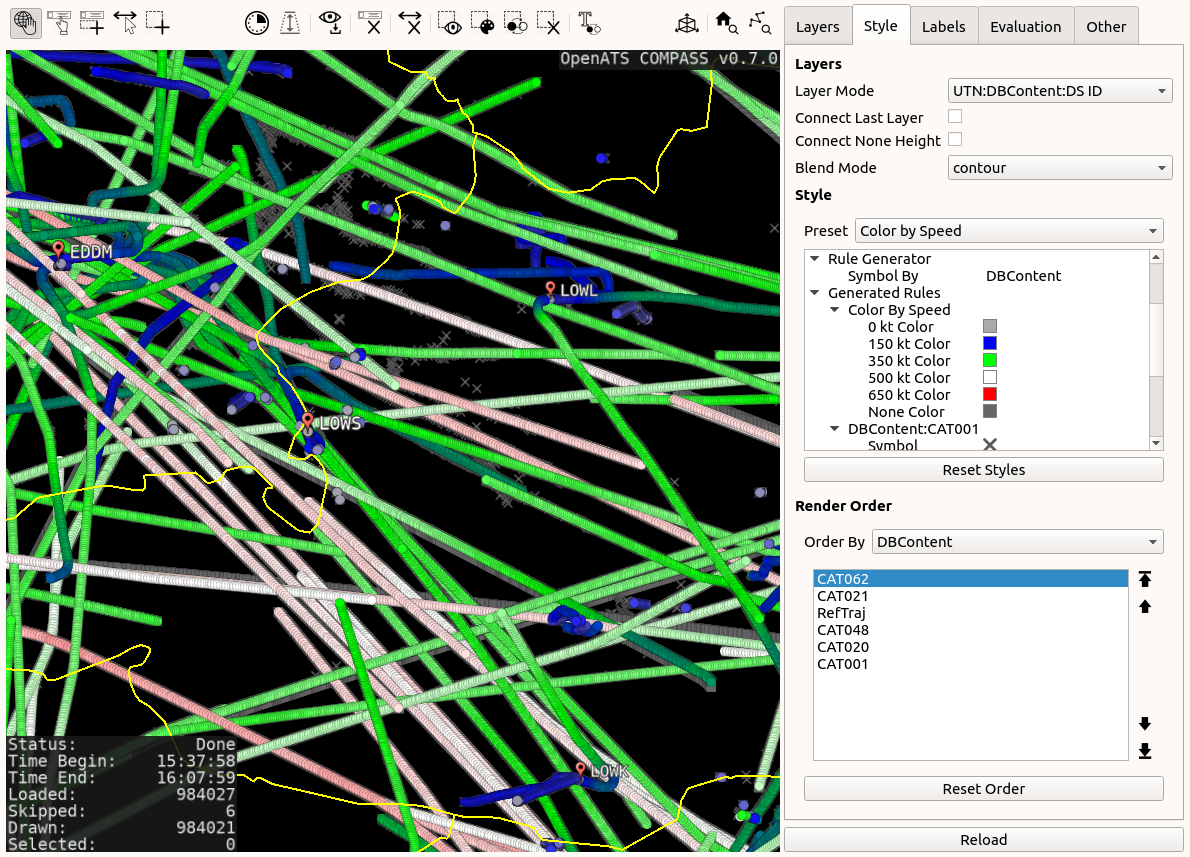
\includegraphics[width=19cm,frame]{../screenshots/osgview_style_speed.png}
  \caption{OSG View Color by speed}
\end{figure}

\begin{figure}[H]
    \hspace*{-2.5cm}
    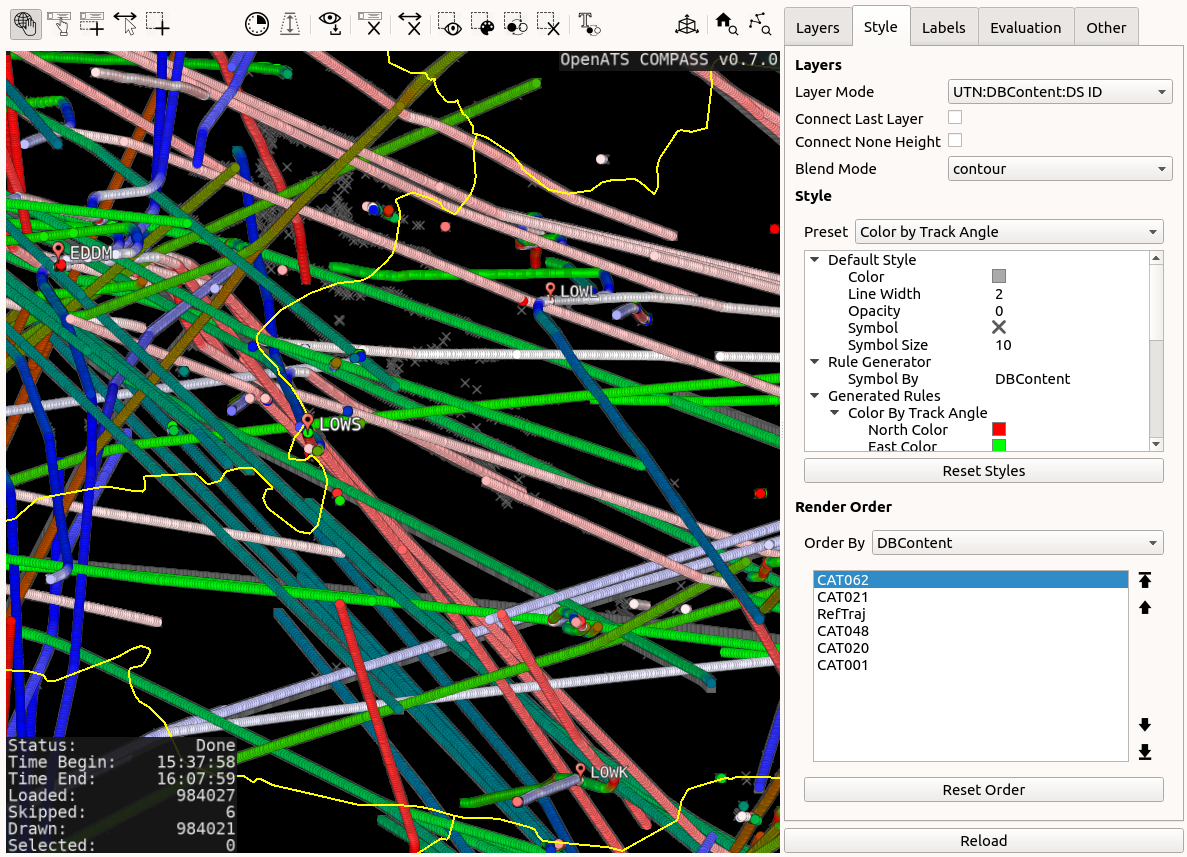
\includegraphics[width=19cm,frame]{../screenshots/osgview_style_track_angle.png}
  \caption{OSG View Color by track angle}
\end{figure}

\begin{figure}[H]
    \hspace*{-2.5cm}
    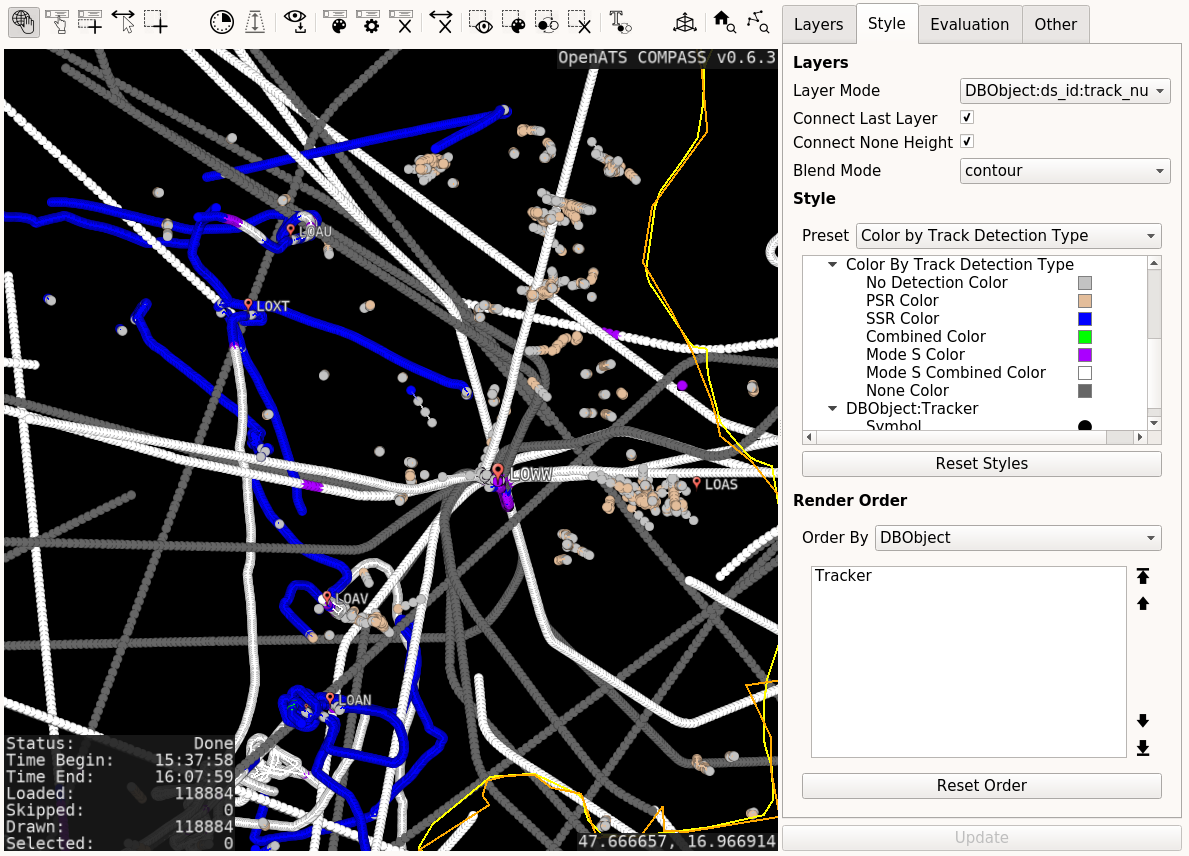
\includegraphics[width=19cm,frame]{../screenshots/osgview_style_tracker_detection_type.png}
  \caption{OSG View Color by tracker detection type}
\end{figure}

Please note that:
\begin{itemize}
 \item The detection type here reflects the technology used to update the track. E.g. an MLAT SSR detection + a PSR detection can form detection type 3 (Combined).
 \item The method used to determine the detection type is slightly different than in Verif
 \item The method used to determine the detection type is currently being discussed/tested by users and will be documented after being accepted.
\end{itemize}

\subsubsection{Render Order}

In the render order widget, the drawing order of the drawn geometry is specified. The one at the top is drawn last (over all others), so it is useful to move the most important DBObject (for the current inspection) to the top.

\begin{figure}[H]
    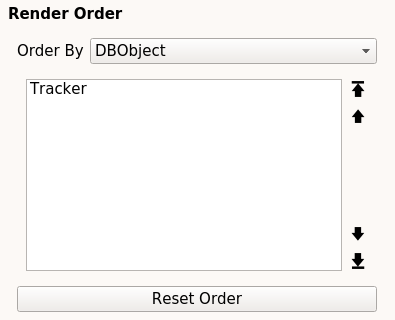
\includegraphics[width=8cm,frame]{../screenshots/osgview_render_order.png}
  \caption{OSG View render order}
\end{figure}

Using the 'Order By' checkbox, the drawing order can be defined based on:
\begin{itemize}
 \item DBObject: Data-source type (e.g. Tracker, Radar, ...)
 \item ds\_id: Data-source (e.g. Tracker1, Tracker2, Radar3, ...)
\end{itemize}
\ \\

To change the drawing order click on the item to move and use the buttons on the right side. Please note that no redraw is required and that the drawing order is persisted in the configuration. \\

 \begin{itemize}
 \item \includegraphics[width=0.5cm]{../../data/icons/top.png} Move to Top: Move item to top position
 \item \includegraphics[width=0.5cm]{../../data/icons/up.png} Move Up: Move item one position up
 \item \includegraphics[width=0.5cm]{../../data/icons/down.png} Move Down: Move item one position down
 \item \includegraphics[width=0.5cm]{../../data/icons/bottom.png} Move to Bottom: Move item to the bottom position
\end{itemize}
